\documentclass[a4paper]{article}
%% Language and font encodings
\usepackage[english]{babel}
\usepackage[utf8x]{inputenc} \usepackage[T1]{fontenc}
\usepackage{amsfonts}
\usepackage{graphicx}
\usepackage{amssymb}
\usepackage{bm}
\usepackage{amsmath}
\usepackage[colorlinks=true, allcolors=blue]{hyperref}
\usepackage{titlesec}
\usepackage{wrapfig,setspace,subfig}
\usepackage[labelfont={bf,it}, textfont=it, justification=centering]{caption}
%% Sets page size and margins
\usepackage[margin=3.5cm]{geometry}
%\usepackage[
%	a4paper,
%	top=3cm,
%	bottom=2cm,
%	left=3cm,
%	right=3cm,
%	marginparwidth=1.75cm
%]{geometry}

%commands
\newcommand{\mat}[1]{\mathbf{#1}}
\newcommand{\vect}[1]{\bm{#1}}
\newcommand{\com}[1]{}

\setlength{\parindent}{0em}
\setlength{\parskip}{8pt}

\titlespacing\section{0pt}{12pt}{2pt}
\titlespacing\subsection{0pt}{12pt}{2pt}

\title{$\vec{E}$mission Individual Report}
\author{2228029M,\\
	School of Physics and Astronomy,\\
	University of Glasgow
}

\begin{document}
\maketitle

\begin{abstract}\noindent
	A large number of physical systems are described by the Laplace
	Equation (LE). In this paper we discuss the development of an
	application to numerically solve the LE for electrostatic problems with
	abstract geometries. The specific contributions made to the group by me
	will be highlighted to give an in depth picture of how they tie into
	the work of the Emission Group\footnote{The name we gave our project
	and group.} as a whole.
\end{abstract}

\section{Introduction}
The purpose of the computation project was to develop a graphical application
capable of solving arbitrarily specified two dimensional problems in
electrostatics. The problem is specified through a drawing area offered by the
custom built GUI, after which it is converted to raw data which can be fed into
two possible subroutines. The first solves the problem iteratively while the
second solves it through direct matrix manipulation. Error analysis was
performed on both methods by comparing them with analytical solutions where
available as well as with each other. The source code was distributed and
integrated using the Git revision control system on a publicly accessible
repository.

\section{Preliminaries}

\subsection{Development Cycle}
Development took place over the course of the semester in a team of five
people. Prototyping was done in MATLAB and then ported to C and C++. The
codebase consists of largely original code with some linking to external
libraries. As mentioned previously, Git revision control was used on the
GitHub platform to facilitate collaboration.  

\subsection{User Interface}
The user interface was developed by one of the team members according to the
criteria set by the project outline. Consequentially, the subroutines in the
back-end had to be tailored to handle the technical restrictions placed on them
by the GUI. The end result was a unique interface that was well integrated with
the numerical solvers that allowed for the easy specification of the
electrostatic geometries.

\subsection{Numerical Solvers}
Two basic numerical solvers were implemented. One was an iterative solver that
utilises successive over relaxation (SOR) and a second which solves the system
directly using LU decomposition. The focus of this report will be the latter as
it was the main area to which my contributions were made.

\section{The Direct Method}
The direct method is possibly the most logically straightforward way to solve
for the values of the mesh points. It involves expressing the relationships of
the various grid points with each other through a system of simultaneous
equations, and then solving this system to obtain a vector containing the
solutions to the mesh points. Thus, in contrast to the iterative methods,
results are obtained at their final accuracy rather than being successively
improved over several cycles.

In our implementation we consider as system of the form:
\begin{align*}
	-4&V_1+V_2+0V_3+0V_4+V_5+\dots+0V_{16}&=0\\
	&V_1-4V_2+V_3+0V_4+0V_5+V_6+\dots+0V_{16}&=0\\
	&\vdots\\
	0&V_1+\dots+V_{12}+0V_{13}+0V_{14}+V_{15}-4V_{16}&=0\\
\end{align*}
Which can be expressed by the matrix equation:
\begin{equation}
	\mat{A}\vect{v}=\vect{b}
	\label{matEq}
\end{equation}
Where $\mat{A}$ is a matrix holding the coefficients of the system, $\vect{v}$
holds the voltage solutions, and $\vect{b}$ represents the right hand values of
the system. We could now apply a variety of generic matrix solving techniques
to find $\vect{v}$ but these methods quickly become impossible to practically
implement in larger problems for reasons discussed in the following sections.

\section{Implementation of the Direct Method}
The first thing to notice is that if we have a $N\times N$ grid then the
coefficient matrix has $N^4$ elements. This quartic growth means that the
storage space required quickly overtakes any realistic memory capacity.
Furthermore, even if one could procure such an expansive memory device, we
would still leave much to be desired in terms of efficiency. To understand why
this is, consider the structure of the matrix $\mat{A}$. We can notice that on
any given line there are at most five non zero elements: the point of interest,
and the four points around it. The rest of the elements on that row are
initialised to zero. The net effect of this is that the matrix $\mat{A}$ is
\emph{extremely} sparse, especially for large $N$. In fact the sparseness of
the matrix is the principle factor on which optimisations are made~\cite{NR}.
In the next section we discuss methods of storing large sparse matrices and the
challenges they present.

\subsection{Storage Systems for Sparse Matrices}
The essential idea behind sparse matrix compression is to minimise the required
storage space by only storing non-zero elements and their respective positions
such that all the information of the original matrix is still preserved.
Although there are several compression schemes available~\cite{101matstore} we
utilised coordinate storage (COO) and compressed column storage (CCS).

The COO storage format is possibly the simplest to understand and implement. It
essentially involves storing three columns or arrays of data: one that tracks
the row numbers of the non-zero elements, another that tracks the column
numbers, and finally one that tracks the values themselves. While this method
offers a fairly good compression rate for large $N$ and is easy to implement,
it does suffer from a few drawbacks. Firstly, it does not optimise on the fact
that several non-zero elements share the same column (or row) number; secondly,
and more significantly, if we wanted to access the non-zero element $v$ with
row number \texttt{i} and column number \texttt{j} we would have to scan
through all the elements preceding it.

To overcome these shortfalls we may use the CCS format. As done previously we
will maintain three data sets, one of which will hold the non-zero values. The
second data set will hold the corresponding row values of those elements.
Finally, the third set holds holds \emph{column offsets} which tell us where in
the value set the next column begins. This not only reduces the space required
but also allows us to \emph{jump} to a requested value by referring to the
column offsets rather than scanning through every element~\cite{101matstore}.

In our code we write in the COO format and use the package
CSPARSE~\cite{csparse} to convert this into the CCS format before solving.

\subsection{Formulating the Linear System}
The system of equations as described thus far holds no information with regard
to any specific geometry and therefore solves no particular problem. Thus, an
essential step is finding a mechanism whereby the system can be tweaked to
reflect a given problem.

To see how this was achieved, consider the $4 \times 4$ grid shown
in Fig.~\ref{gridFig} with a voltage of 25V at $v_6$. How can this information
be represented in the system? The solution employed was to zero out the row
corresponding to $V_6$ (row 7 if we index from 0) and write a 1 into its
diagonal. We then write 25 in the corresponding element of the $\vect{b}$
vector. The reason this works can be seen by multiplying out the left hand side
of~\eqref{matEq}. Notice that all the zero elements in row 7 will ensure almost
all the variables disappear, leaving only the 1 in the diagonal to be
multiplied to yield the equation $v_6=25$ which is precisely the restriction we
wished to specify.
%Figure of the 4x4 grid.
\begin{figure}
  \centering
\subfloat[]{\includegraphics[width=0.3\textwidth]{4x4grid2.png}\label{gridFig}}
  \hfill
  \subfloat[]{\includegraphics[width=0.5\textwidth]{stencils}\label{stencils}}
  \caption{(a)An example of a $4 \times 4$ grid. (b) Some incarnations of the 
stencil at various points on the grid}
\end{figure}

To deal with the boundaries we use a method we shall call \emph{adaptive
stencilling}\footnote{This is a fairly simple modification of the five point
star, but at the time of writing we failed to find reference or utilisation of
it in the scientific literature.}. The idea is to adapt the number of
\emph{legs} of our stencil as we crawl the mesh depending on where we are;
changing from a three point stencil to a four point one when we are at the
corners or the sides respectively. Without this modification, every time we
wish to calculate a point on the side of the grid (e.g. $v_{11}$ in
Fig.~\ref{gridFig}) we end up dividing by 4 even though we only have 3
neighbours. Thus it is as if we have assumed there to be a fourth point that is
always 0. The net result of this is the boundaries are fixed at nearly zero
which, needless to say, is in general incorrect.

\begin{figure}
  \centering
\subfloat[]{\includegraphics[width=0.5\textwidth]{fixedboundary}\label{fxbound}}\hfill
\subfloat[]{\includegraphics[width=0.5\textwidth]{adaptiveboundary}\hfill
\label{adbound}}
  \caption{Results with and without adaptive stencilling respectively. Notice 
how the boundaries are no longer fixed at zero.}
\end{figure}

Now that the matrix can be stored and tailored to our problems we can explore
how the system is solved.

\subsection{Solving the Linear System}
Since taking full advantage of a CPU through efficient symbolic manipulation of
the matrices, and linking the algorithms to a specialised linear algebra
library is a very challenging task, we decided to utilise the SuperLU package
for solving.

To explain how SuperLU works we will break up the stages of the simplest
algorithm it employs to solve a Eq.~\eqref{matEq}. The stage 1
concentrates on memory and the stage 2 on speed.

As mentioned earlier the matrix A is a very large, asymmetric and sparse  
matrix so we store it in CCS form. This however would pose a problem since 
computing simple LU decomposition would result in dense L and U matrices, 
instantly defeating the purpose of storing A in CCS format. This is treated by 
SuperLU in part 1 of the following algorithm called `Simple Driver Algorithm'
seen underneath.

Compute $P_rAP_c = LU$ where $P_r$ is a permutation matrix which reorders the 
rows and $P_c$ reorders the columns. $L$ is a unit lower triangular matrix and
$U$ an upper triangular one.
$P_c$ is chosen to order the columns of $L$ and $U$ to increase their sparsity. 
This is done by making use of another data structure called supernodes. 
Supernodes group together columns with the same non-zero structure thus 
conserving space. It makes sense then that to maximise the effectiveness of 
supernodes we permute the matrix to bring together columns with the same 
non-zero structures. This can be done without destroying important 
information by a post-ordering on $\mat{A}$'s column elimination tree \cite{ref27}
which is computed in time almost directly proportional to the number of
non-zero entries \cite{ref35}, giving us $P_c$. SuperLU can then perform
dynamic pivoting and row-interchanging to simultaneously find the LU
factorisation of $P_c$, $\mat{A}$ and $P_r$.

Eq.~\eqref{matEq} can therefore be solved via
$X = \mat{A}^{-1}\vect{b}= (P_r^{-1}LUP_c^{-1})^{-1}\vect{b} =
P_c(U^{-1}(L^{-1}(P_r(B))))$
corresponding to a permutation of the rows of $\vect{b}$, followed by solving a
number of triangular systems equal to the entries in $\vect{b}$ by substitution.
Similarly, followed by solving the same number of triangular systems, to obtain
an answer for $\vect{v}$ without explicitly computing the inverse of $\mat{A}$.

\section{Performance of the Direct Method}
We evaluated various metrics to gauge the performance of the algorithm. First
we measured execution time with image size (see Fig.~\ref{sizetestFig}).
\begin{figure}
	\centering
	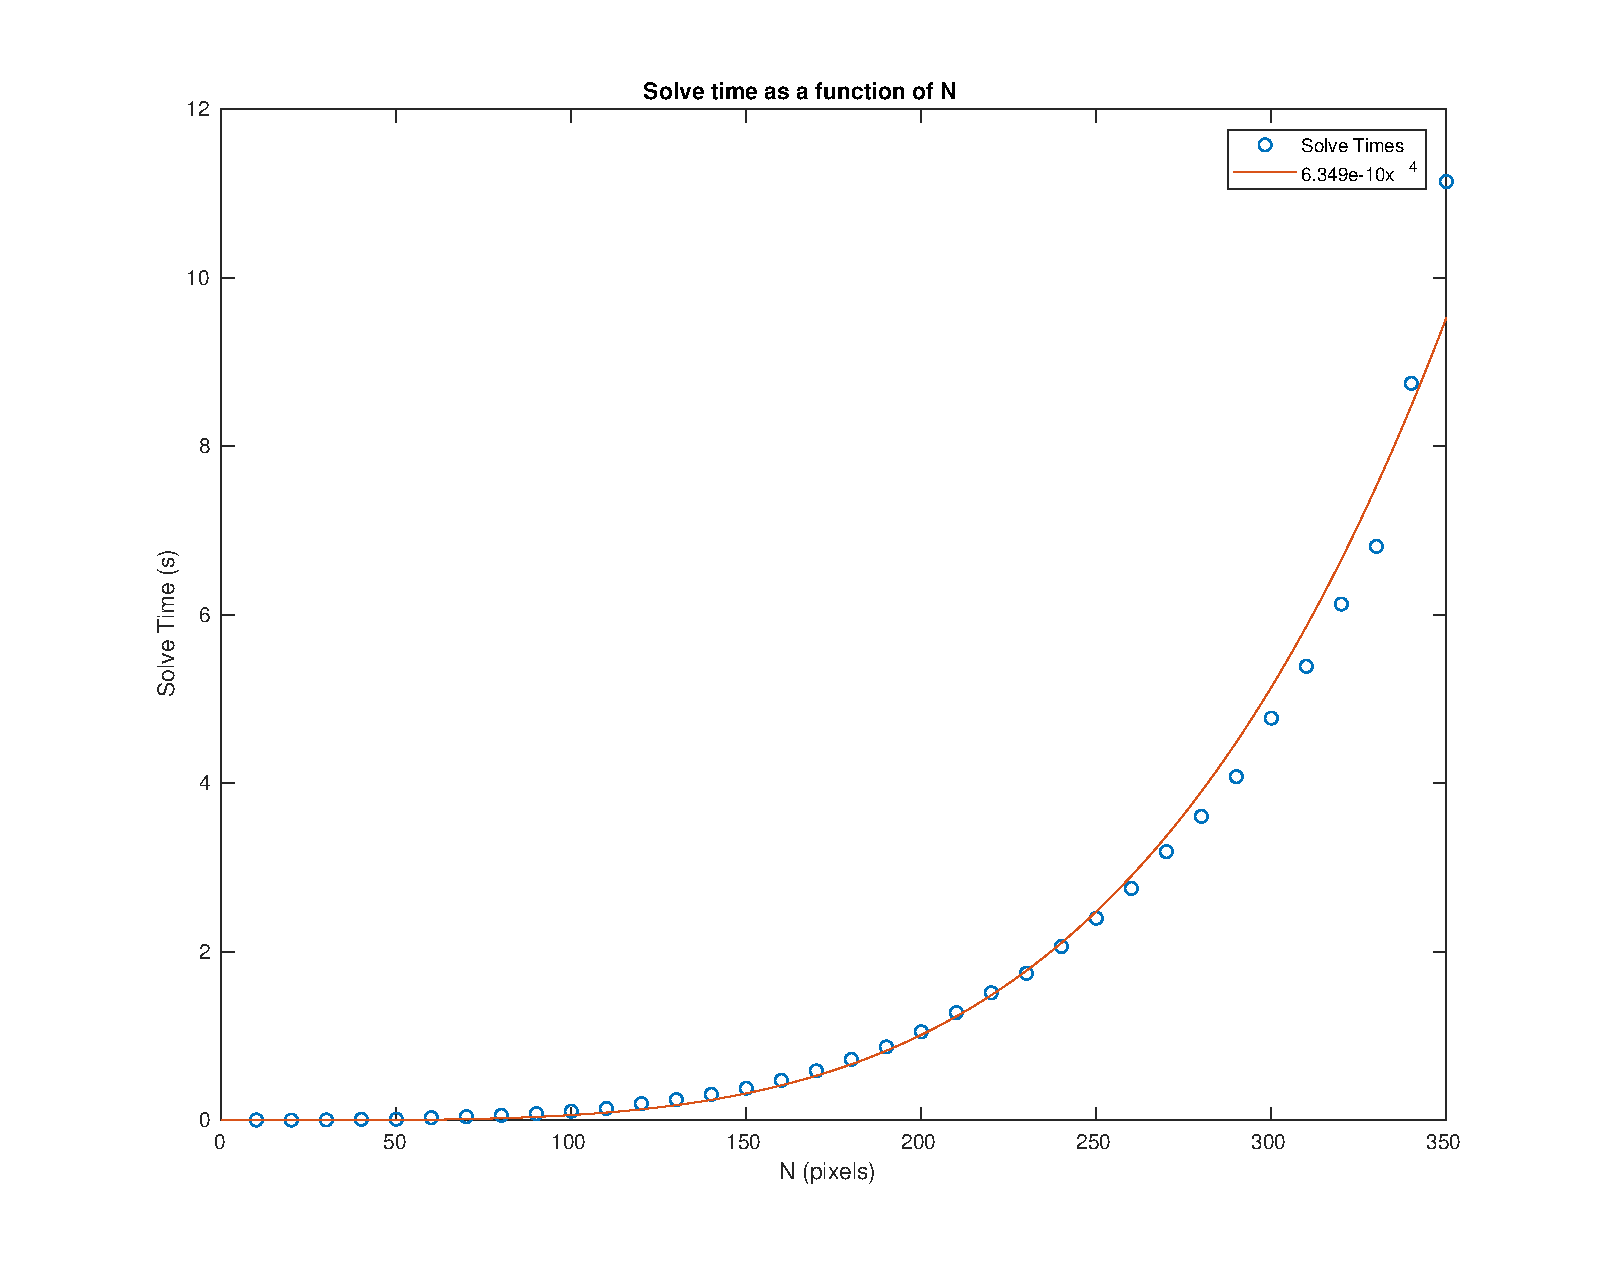
\includegraphics[scale=0.21]{sizebenchmark.eps}
	\caption{Variation of the solve time (in seconds) to $N$. The data fits
	quite well to a $N^4$ curve which is to be expected as this is the rate
	at which the matrix grows.}
	\label{sizetestFig}
\end{figure}
The code was tested with the same image at various sizes and the results were
plotted. Although exact solve times vary depending on the specific geometry,
the general trend should be the same.

Error was analysed by comparing the analytical results of Problem~0 and
Problem~1. For each pixel an absolute difference of the values was calculated
and we were able to use this to calculate the relative error of the numerical
solution.
        
\section*{Conclusion}
Conclusion.

\pagebreak
\bibliographystyle{alpha}
\begin{thebibliography}{15}

	\bibitem{NR}
		\emph{Numerical Recipes: The Art of Scientific Computing}\\
		W. H. Press, S. A. Teukolsky, W. T. Vetterling, B. P. Flannery\\
		September 2007\\
		ISBN: 9780521880688

	\bibitem{101matstore}
		\emph{101 Ways to Store a Sparse Matrix}\\
		Max Grossman\\
		\texttt{https://medium.com/@jmaxg3/101-ways-to-store-a-sparse
		-matrix-c7f2bf15a229}\\
		Accessed: 12\textsuperscript{th} March 2018
        
	\bibitem{matrixcomp}
		\emph{Fundamentals of matrix computations,  second edition}\\
		David S. Watkins\\
		2002

	\bibitem{omega}
		\emph{The optimal relaxation parameter for the SOR method
		applied to the Poisson equation in any space dimensions}\\
		Shiming Yang, Matthias K. Gobbert\\
		2008

	\bibitem{vonNeumann}
	\texttt{https://www.12000.org/my\_courses/UC\_davis/fall\_2010/math\_228a/HWs/HW3/Neumman\_BC\\
	/Neumman\_BC.htm}
            
	\bibitem{stop}
  		\verb!http://ta.twi.tudelft.nl/users/vuik/burgers/lin_notes.pdf!
  
	\bibitem{ref27} 
		\emph{R. Gilbert and E. Ng, Predicting structure in 
		nonsymmetric sparse matrix factorizations,
		in Graph Theory and Sparse Matrix Computation}\\
		A. George, J. R. Gilbert, and J. W. H. Liu, eds.,\\
		Springer–Verlag, New York, Berlin, 1993.
    
	\bibitem{ref35}
		\emph{The role of elimination trees in sparse factorization}
		J. W. H. Liu

	\bibitem{qtref}
		\emph{Qt Documentation}\\
		\texttt{http://doc.qt.io/qt-5/reference-overview.html}

	\bibitem{csparse}
		\texttt{
		https://github.com/PetterS/SuiteSparse/tree/master/CSparse 
		}
\end{thebibliography}
\end{document}
